\subsection{Howell Coward}
\begin{table}[h]
  \centering
  \begin{tabular}{l||c|c|c|c|c|c|c|c|c}
    Model & log$_{10}\left(L_* \left[ \text{erg} \text{ s}^{-1} \right] \right)$
& $\alpha$ & $\beta$ & $\rho_0 \left[\text{Gpc}^{-3} \text{ yr}^{-1} \right]$ &
$z_1$ & $n_1$ & $n_2$ & $N_\text{GRB}$ \\
    \hline
    WP & 52.53 & 0.17 & 1.44 & 1.25 & 3.11 & 2.07 & -1.36 & 9082.83\\
%     HC 1 & 51.9 & 0.95 & 2.59 & 0.48 & 3.6 & 2.1 & -0.7 & 4791.97\\
    HC & 51.7 & 0.13 & 2.42 & 0.48 & 3.6 & 2.1 & -0.7 & 4791.97\\
  \end{tabular}
  \caption{Fit parameters to the luminosity functions and redshift
distributions of the tested models.}
  \label{tab:grb_model_params}
\end{table}
There is a more recent work (reference ???) by Howell, Coward, Stratta,
Gendre and Zhou basing the redshift distribution on
(rerference ???) and testing various luminosity functions. For purposes of
readability it will be called Howell-Coward or HC-model. 
One of the tested luminosity functions
will be compared to the model by Wanderman and
Piran. 
%They are designated HC1 and HC2.

Similarly to Wanderman and Piran, the luminosity is assumed to not evolve
with redshift in their main work.
The same functions as in WP are used for redshift distribution (eq. 
\ref{eq:R_z}) and the
luminosity function (eq. \ref{eq:Phi_L}), but different fit results
were obtained for the parameters (Table \ref{tab:grb_model_params}).

The considered luminosity range is with $\text{log}_{10} L_\text{Peak} \in
\left( 49, 54 \right)$ larger than in WP ($\text{log}_{10} L_\text{Peak} \in
\left( 50, 54 \right)$). The break peak luminosity is lower
than in WP transitioning into a harder slope towards higher luminosities (Fig.
\ref{fig:wp_hc_comp}). At lower luminosities the slopes of HC and WP are
quite similar (0.13, 0.17) leading to more low luminosity GRBs in HC due to the 
greater range.

% The redshift distribution in HC is shifted to smaller values of $R(z)$ as a
% smaller local rate and total number of GRBs is assumed (Table
% \ref{tab:grb_model_params}). 
The redshift distributions rise to the break redshift quite similarly though 
the break is at higher redshifts (3.6 compared to 3.11) for HC transitioning
into a slower decay at large $z$. The overall impact are more distant GRBs in
HC than in WP which should lead to a slight weakening of the limits.

\begin{figure}[ht]
% [htb] 
\subfloat[Luminosity functions\label{fig:wp_hc_comp_lum}]
{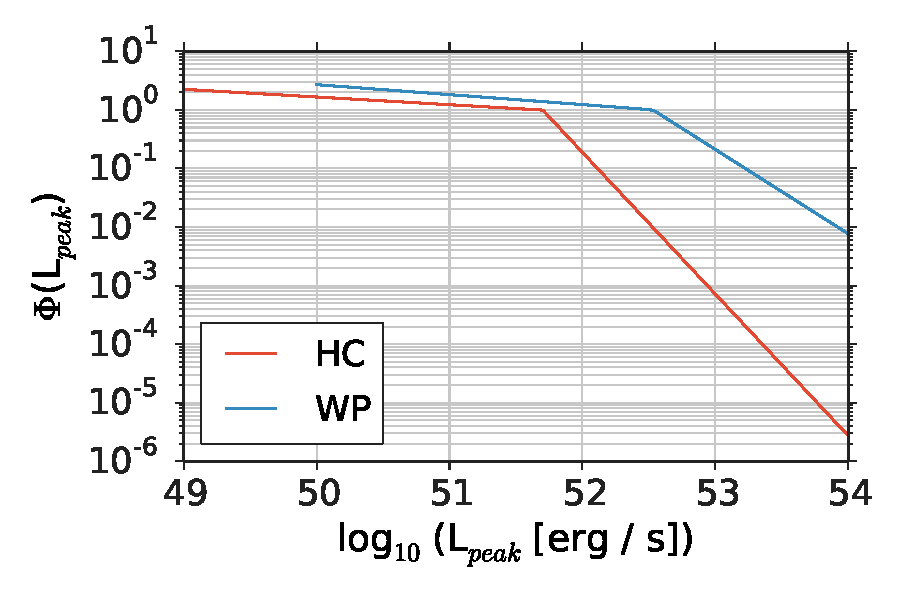
\includegraphics[width=0.48\textwidth]{fig/grb_models_lum_comp_L45.pdf}}
    \hfill
\subfloat[Redshift distributions\label{fig:wp_hc_comp_z}]
{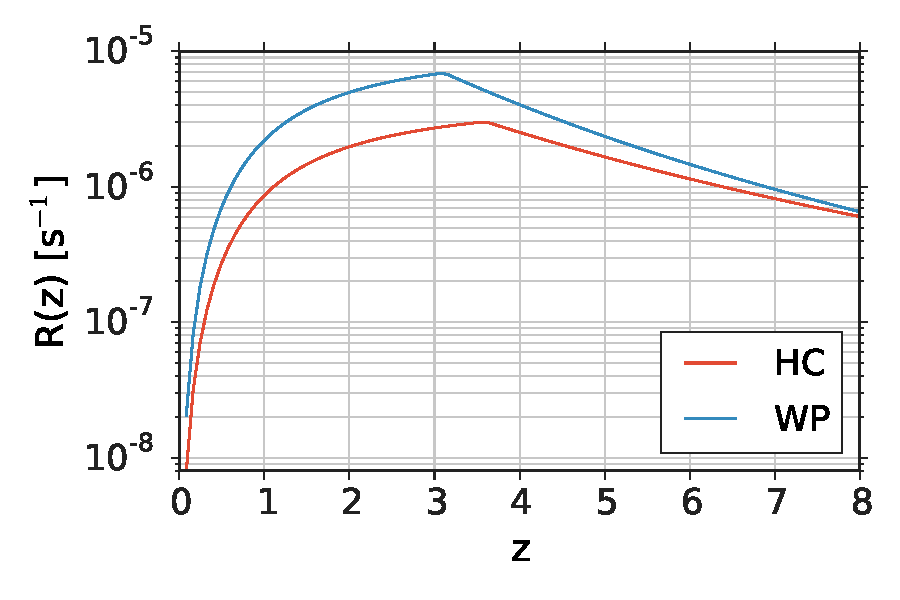
\includegraphics[width=0.48\textwidth]{fig/grb_models_redshift_comp.pdf}}
    \caption{The luminosity functions (left) from the
Wanderman-Piran model and two functions from the HC model on the left. The WP
only take into account luminosities in the range of $10^{50} - 10^{54}$ erg / s
which is reflected in the shorter blue line.\\
The redshift distributions (right) develop similar up to $z=3.11$ at which point
it breaks for the WP-model. The HC predicts more GRBs at higher redshift
values.}
\label{fig:wp_hc_comp}
\end{figure}


% While most of cases discussed in (reference ???) imply independentend luminosity
% and redshift, a correction is given to examine the influence of a possible
% evolution. This will be added at a later point as a third comparison model.